\section{作业及答案：结构力学基础与技巧班第9次作业及答案（静定结构位移计算）}
\begin{analysisbox}
位移计算以虚功原理为核心。常用单位荷载法、图乘法和积分法，关键是实结构内力图与虚结构内力图的符号和区段对应。
\end{analysisbox}
\subsection*{第 1 页转写}
六、练习题

4-1图4-43所示结构中截面A转角（设顺时针为正）为（

）。（哈尔滨工业大学

2009)

A.2Fpa?/EI

B.-Fpa?/EI

C.5Fpa /(4EI)

D.-5Fpa /(4EI)

4-2图4-44所示悬臂梁，B点的竖向位移为

（合肥工业大学2010）

Fp-ql

2EI

EI

EI

图4-43

图4-44

4-3图4-45所示桁架，C点的水平位移（）。（西南交通大学2008）

B.向右

A.向左

152
\begin{figure}[H]\centering
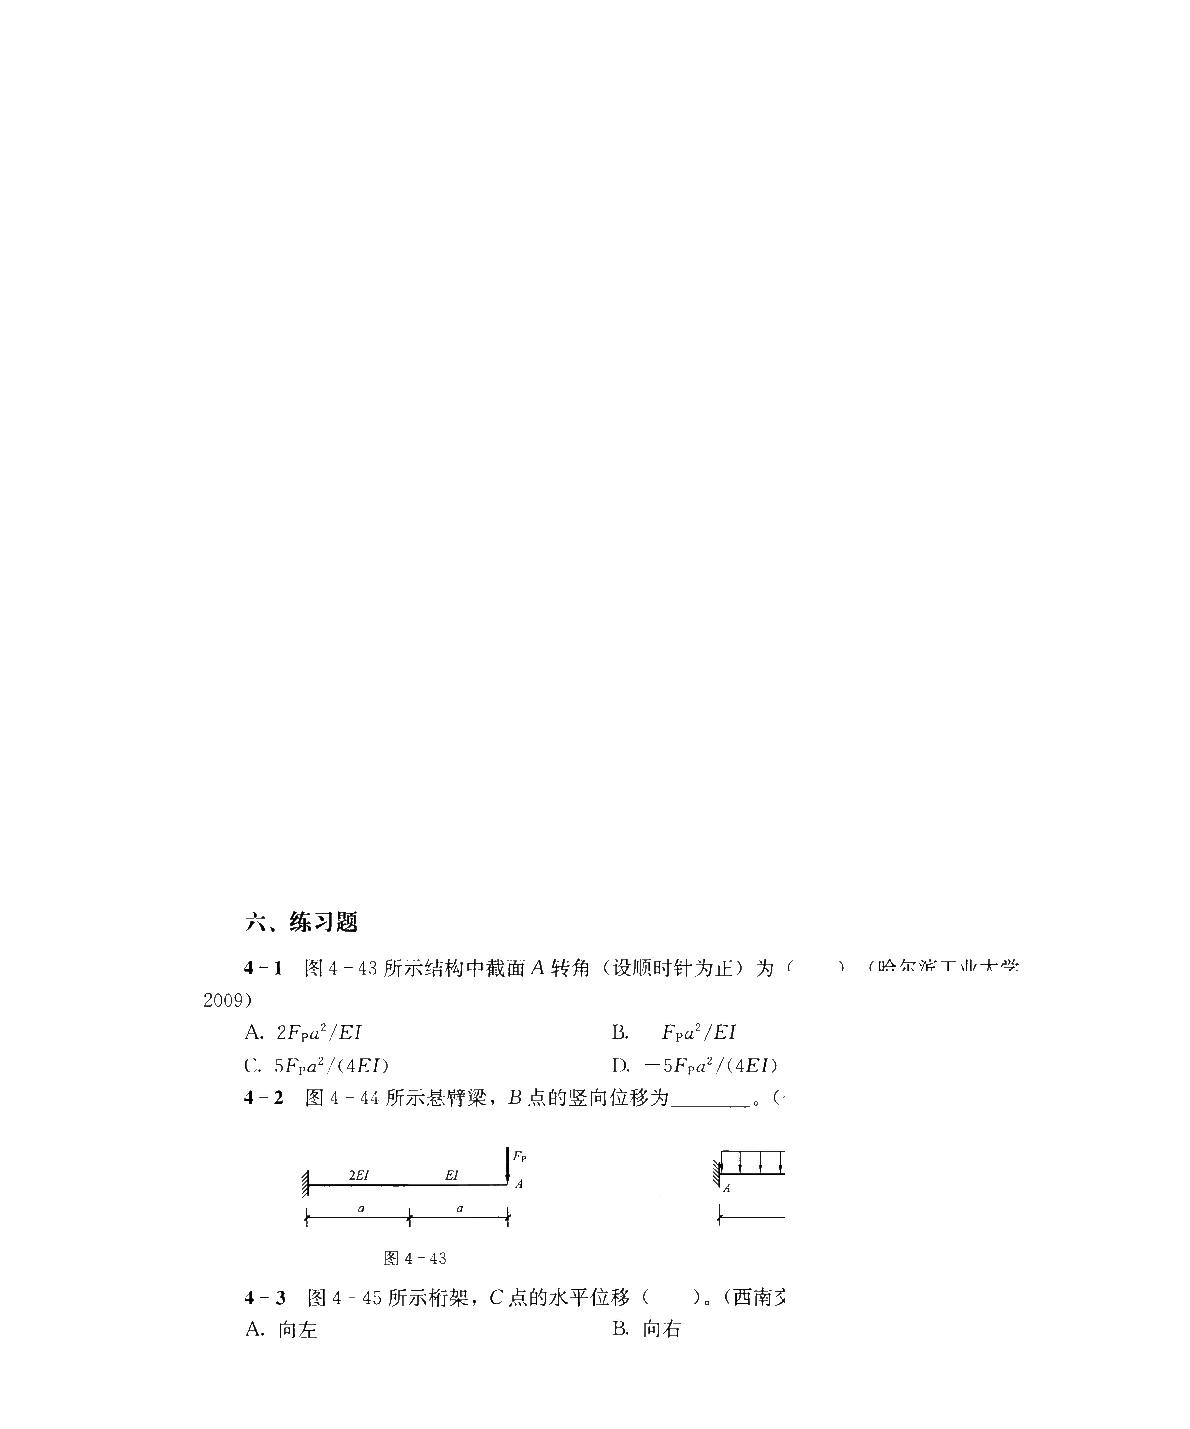
\includegraphics[width=0.92\textwidth]{figures/src12_p001.jpg}
\caption{结构力学基础与技巧班第9次作业及答案（静定结构位移计算） 第 1 页清理图形页}
\end{figure}
\subsection*{第 2 页转写}
永共微倍包7888

C.等于零

D.不定，取决于A/A2的值

图4-46所示刚架中，C、D两点的相对线位移等于

4-4

，两点距离

（河北工业大学2010）

图4－47所示桁架，各杆拉伸刚度为EA，DC杆的转角为

4-5

（天津大学

2010)

EI

EAI

EA2

图4-45

图4-46

图4-47

4-6求图4-48所示结构A、B两点的相对水平位移，EI=常数。（中南大学2012）

4-7画出图4-49所示结构的弯矩图，并求C点的水平位移。设各杆EI相同，且忽

略其轴向变形。（湖南大学2012)

4-8试求图4-50所示结构中截面B左右两侧的相对转角。EI=常数。（福州大学

2010)

FpttFp

10kN/m

20kN

4m

4m

2m

图4-48

图4-49

图4-50

4-9

已知图4-51所示桁架各杆温度上升t ，材料的线膨胀系数为$\alpha$。试求K点的

竖向位移。（福州大学2012）

4-10

计算图4-52所示结构中A、B两点相对水平线位移，EI=常数。（华南理工大

学2012）

4- 11

计算图4－53所示荷载作用下的静定桁架。（1）求各杆轴力；（2）求结构C点

的水平位移$\triangle$Hc和竖向位移$\triangle$vc。已知：各杆截面相同，即EA=常数。（长安大学2008）

FP

qa

3mx4

图4-51

图4-52

图4-53
\begin{figure}[H]\centering
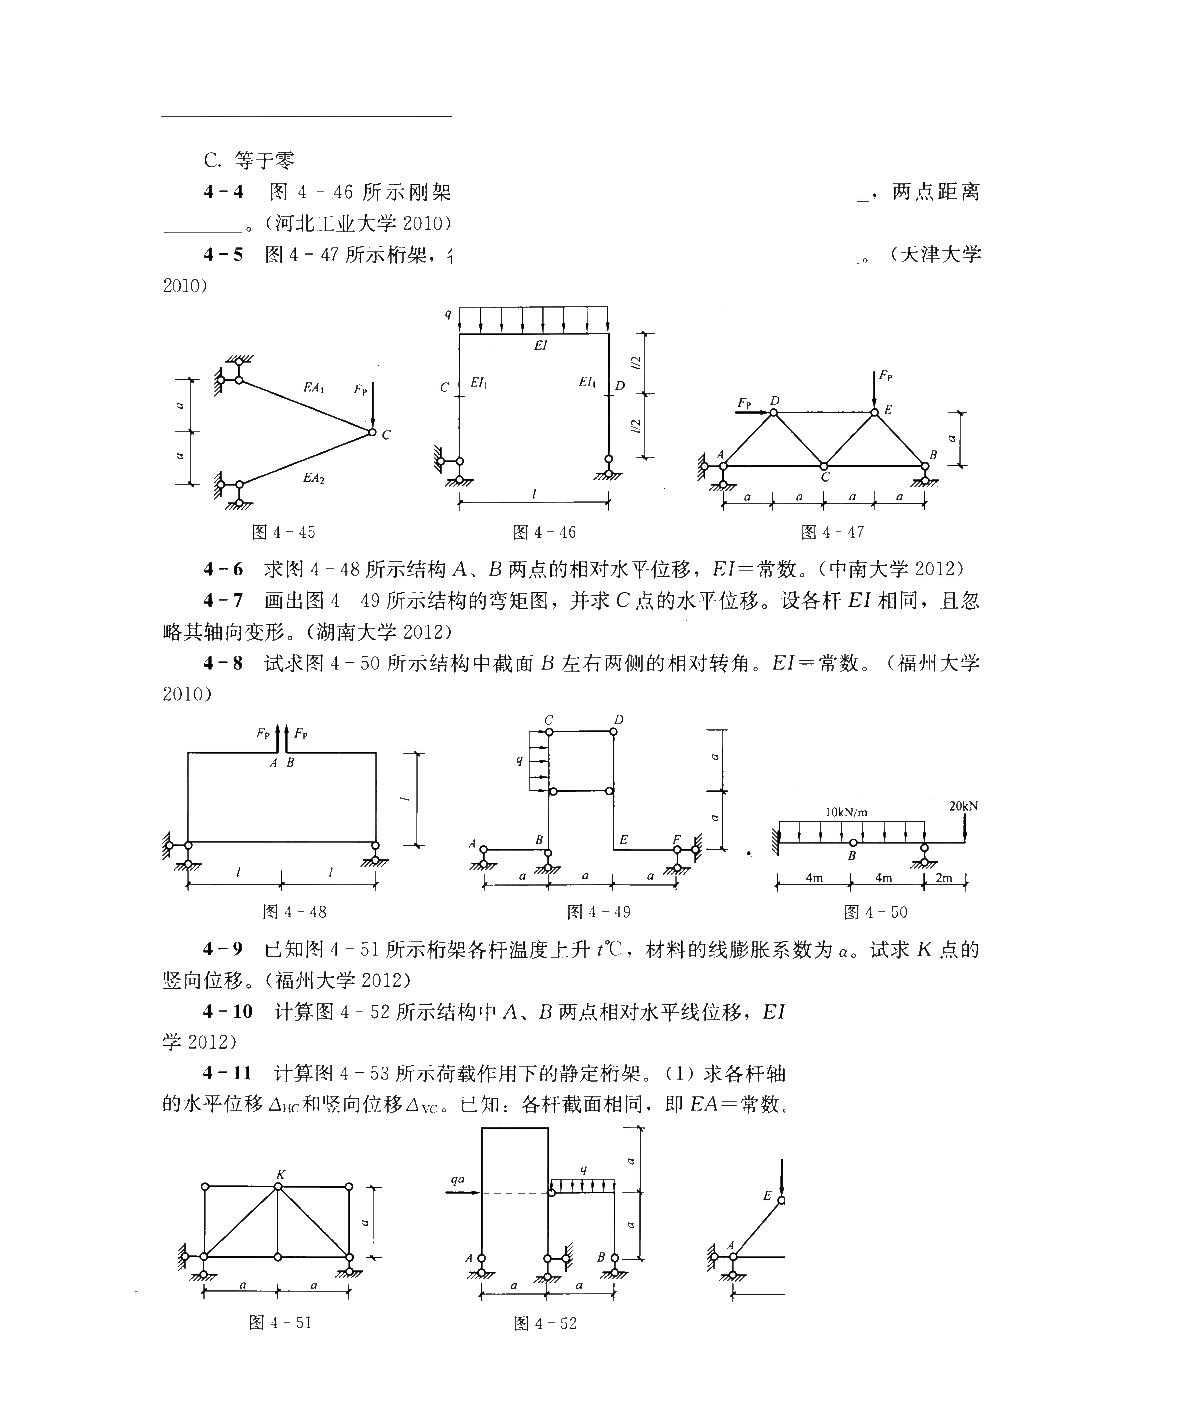
\includegraphics[width=0.92\textwidth]{figures/src12_p002.jpg}
\caption{结构力学基础与技巧班第9次作业及答案（静定结构位移计算） 第 2 页清理图形页}
\end{figure}
\subsection*{第 3 页转写}
研究生入学考试辅导丛书结构力学（第二版）

4-12图4-54所示结构由于支座A沉降1cm引起截面C的转角Oc=

庆大学2012)

4-13图4-55所示多跨静定梁支座A发生线位移a=10mm，转角位移g=0.001rad，

图中[=10m，则铰B两侧截面的相对转角为

，（中南大学2009）

4m

L2m

图4-54

图4-55

4-14

计算图4-56所示结构由于支座移动产生的铰C的角位移。（湖南大学2008）

4-15求图4-57所示结构A点竖向位移$\triangle$vA，EI=常数。（西南交通大学2007)

k-ELP

0.01m

4m

2m

图4-56

图4-57

七、练习题答案

4-1

C.

11g

4-2

(+)。

24EI

4-3

D.

676

4-4

增大。

24ET:

(2+/2)Fp

4-5

2).

2EA

3Fp73

4-6

AAB

EI

)。

67qa4

4- 7

弯矩图如图4-58所示，$\triangle$Hc

(-)。

12EI

320

4-8

(0.

4-9

一$\alpha$ta（个)。

91qa

( )。

4-10

24EI

9Fp

各杆轴力如图4-59所示。AHc=

4 - 11

(- )；$\triangle$vc=0（由反对称荷载下位移的

4EA

154
\begin{figure}[H]\centering
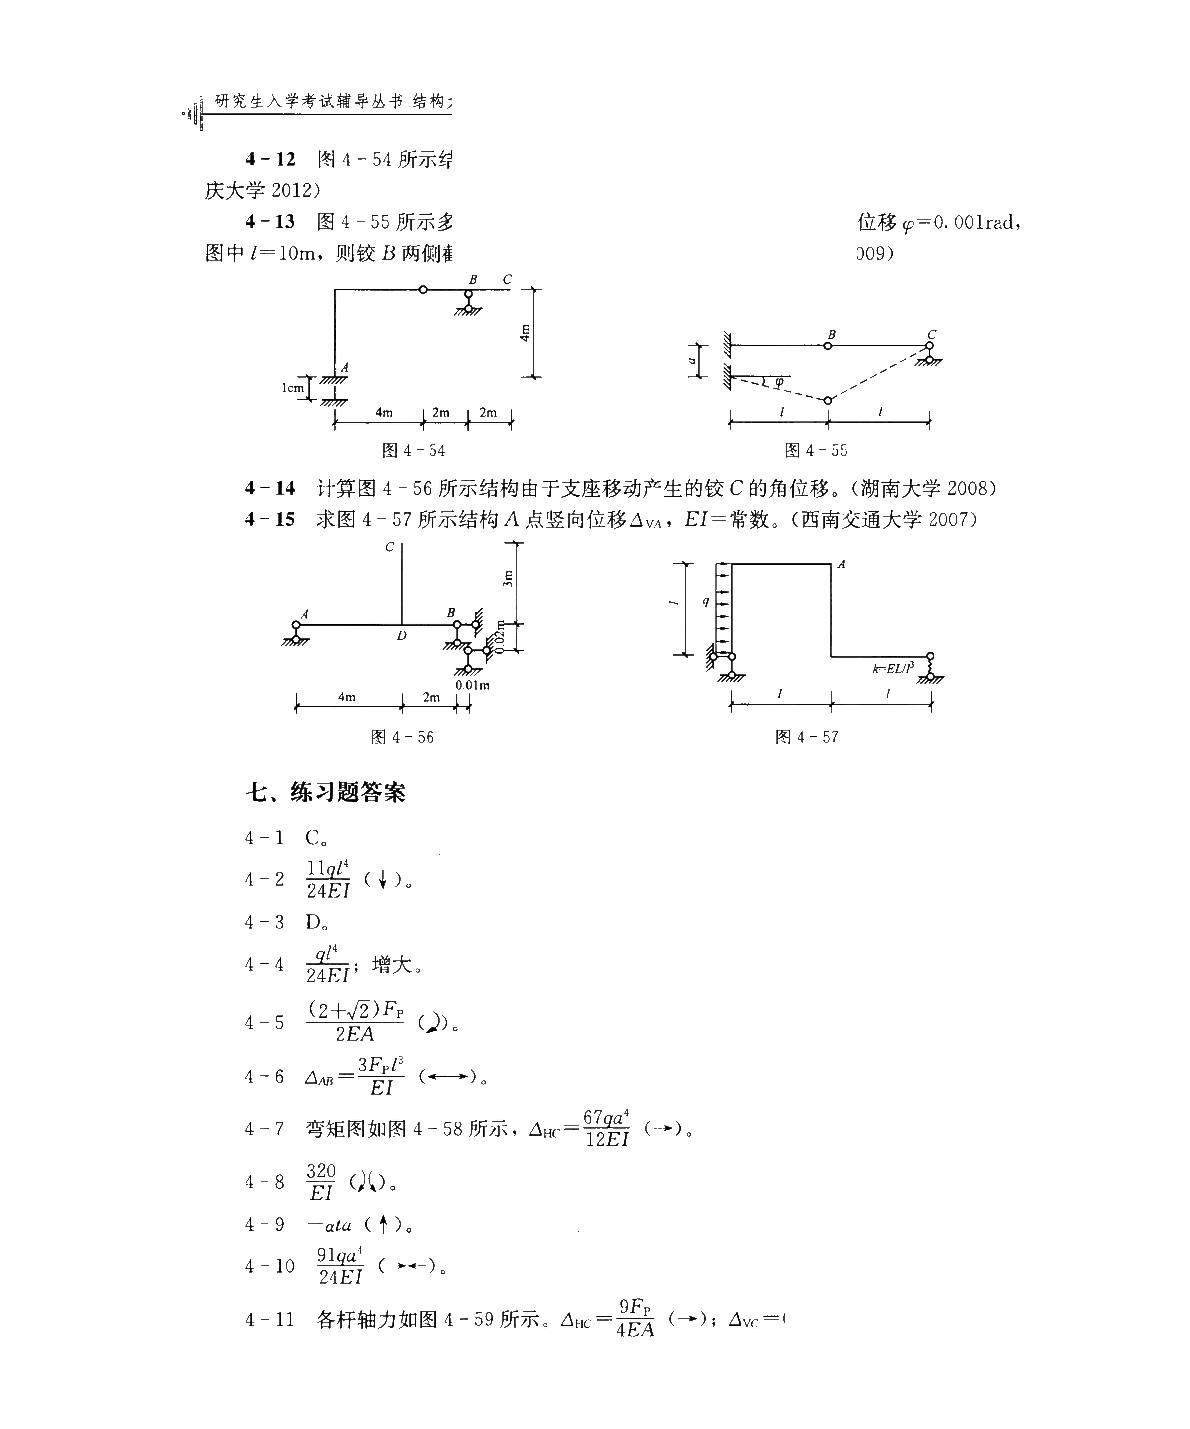
\includegraphics[width=0.92\textwidth]{figures/src12_p003.jpg}
\caption{结构力学基础与技巧班第9次作业及答案（静定结构位移计算） 第 3 页清理图形页}
\end{figure}
\subsection*{第 4 页转写}
特点判断)。

FNCD=qa

Fn--2qa

1.5qd

1.5qd

1.5qq

M图

FNP

图4-58

图4-59

4-12

0.005rad ()。

4-13

0.003rad ())。

4-14

pc=0. 003 3rad (2)。

$\triangle$vA

4-15

(v).

8EI
\begin{figure}[H]\centering
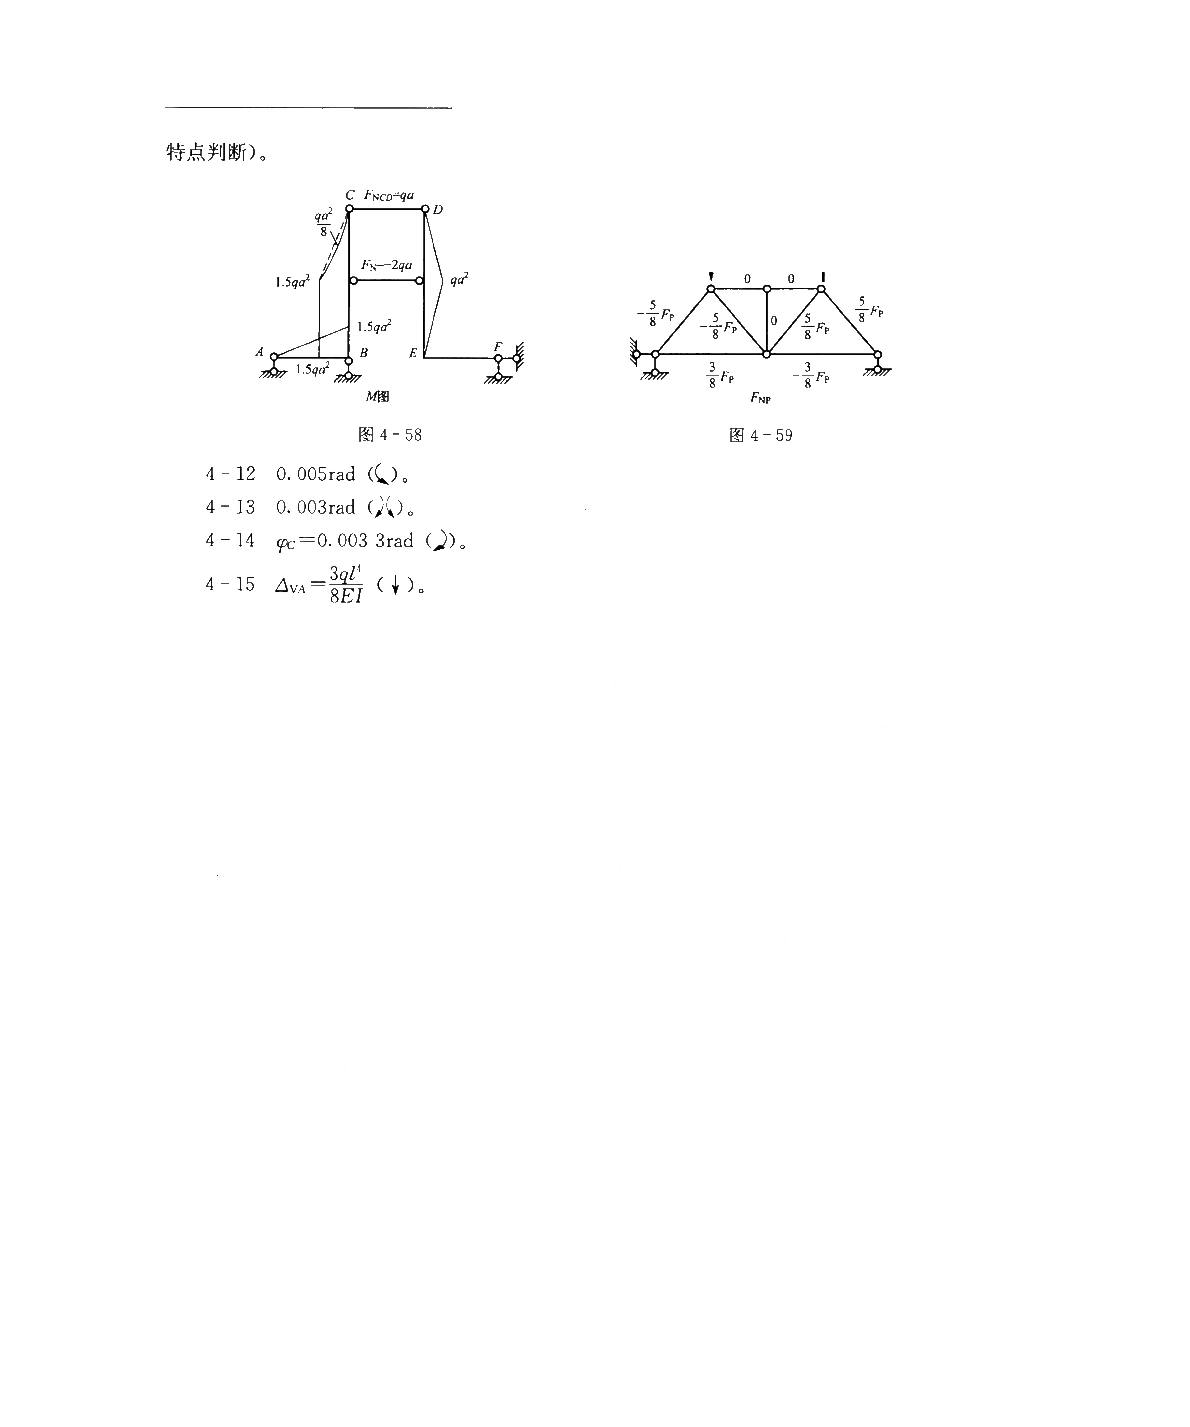
\includegraphics[width=0.92\textwidth]{figures/src12_p004.jpg}
\caption{结构力学基础与技巧班第9次作业及答案（静定结构位移计算） 第 4 页清理图形页}
\end{figure}
